\chapter{Analiza stylu jazdy}

\section{Wstęp}

Niniejszy rozdział stanowi opis dodatkowej funkcjonalności, stanowiącej analizę stylu jazdy kierowcy, oferowanej w zaprojektowanym w pracy urządzeniu. Zawarte są w nim autorskie badania, krótki opis istniejących rozwiązań oraz propozycja własnego algorytmu oceny sposobu jazdy wraz z jego rezultatami. 

Funkcjonalność opisująca styl jazdy jest niezwykle istotna z punktu widzenia jednej z grup docelowych, do których kierowane jest urządzenie - firm posiadających flotę pojazdów. Dzieje się tak, ze względu na rosnące koszty prowadzenia działalności oraz użytkowania pojazdów (wzrost cen paliwa, części zamiennych i usług, a także niezbędnych ubezpieczeń OC) co wprowadza konieczność ograniczenia zbędnych wydatków. Można do nich zaliczyć nadmiernie szybkie zużycie części eksploatacyjnych jak na przykład klocki hamulcowe czy opony, a także koszty związane z wypadkami losowymi takimi jak stłuczki. W przypadku firm, są one często generowane przez nieodpowiedzialnych pracowników, którzy nie szanują własności pracodawcy i prowadzą pojazdy w sposób lekkmyślny, agresywny. Ograniczenie tego procederu jest o tyle problematyczne, iż trudno o jednoznaczne dowody winy pracownika - kierowcy. Odpowiadając na tę potrzebę rynkową, opisywany w tej pracy system umożliwia nie tylko ocenę stylu jazdy i jego zdalny podgląd na bieżąco, lecz także zapisywanie historii ocen przypisanych do punktów przebytej przez pracownika trasy wraz z dodatkowymi parametrami, opisywanymi we wcześniejszych rozdziałach. Pozwala to nie tylko na wskazanie, iż pracownik jechał nadto agresywnie, lecz także informację kiedy i gdzie to nastąpiło.

\section{Istniejące metody}

W ramach przygotowania do implementacji algorytmu analizy stylu jazdy, dokonano przeglądu artykułów opisujących różne istniejące już metody. Najciekawszy z nich (\cite{driving_analysis_article}) opisuje wykorzystanie telefonu typu smartphone jako platformy czujników pomiarowych. Metoda opisana w artykule jest bardzo podobna do sposobu wykrywania gestów w kontrolerach ruchu dedykowanych do gier.  Wykorzystywane są w tym celu dane z akcelerometru oraz żyroskopu oraz system GPS. Pierwsze dwa z nich umożliwiają wykrycie łagodnych i ostrych skrętów, manewru zawracania, a także przyspieszania i hamowania zarówno gwałtownych, jak i spokojnych. Moduł GPS służy do uzyskania informacji o prędkości pojazdu. Głównym algorytmem wykrywania jest DTW (\textit{ang. \textbf{D}ynamic \textbf{T}ime \textbf{W}arping}), który służy do wyznaczenia miary podobieństwa pomiędzy dwoma sygnałami. 
Pierwszym krokiem w zastosowaniu algorytmu jest kalibracja telefonu. Autorzy umieszczają telefon na desce rozdzielczej i odpowiednio go orientują względem pojazdu. Działający na nim program dokonuje filtracji danych filtrem dolnoprzepustowym o częstotliwości 25 Hz ze względu na drgania pochodzące od pracującego silnika. Dane pozyskiwane są w postaci zbioru kilku tysięcy próbek. 
Pierwszym etapem jest wykrycie rozpoczęcia manewru. W tym celu wykorzystano średnią kroczącą:

\begin{equation}
	SMA = \frac{g(i)^2 + g(i-1)^2 + ... + g(i-k-1)^2}{k}
\end{equation}

gdzie
$g(i)$ - wartość próbki przyspieszenia
$k$ - liczba próbek w oknie sygnału

Skok cyklicznie wyliczanej w ten sposób średniej powyżej założonego przez autorów progu traktowany jest jako początek manewru. Trwa on dopóki SMA nie spadnie poniżej progu końca manweru. Jeśli czas trwania ruchu wykrytego w ten sposób jest dłuższy niż 15 sekund, jest on traktowany jako błąd pomiaru i odrzucany.

Wykryte w ten sposób manewry poddawane są następnie przetwarzane przez algorytm DTW. Pozwala on na znalezienie najmniejszej odległości między dwoma sygnałami, czyli stopnia ich podobieństwa. Innymi słowy, w pamięci programu zapisane są pewne uśrednione modele wszystkich wykrywanych manewrów, z którymi porównywane są aktualnie przetwarzane dane. 

Metoda ta pozwala na wykrycie wielu różnych manewrów, lecz jest kosztowna obliczeniowo i pamięciowo, co stanowi kluczową kwestię w systemach wbudowanych posiadających niewielkie zasoby. Ponadto, problemem jest brak precyzyjnej definicji czym jest manewr łagodny, a czym gwałtowny, a bazowanie na swobodnie wybranych modelach.  W związku z tym, bazując na podstawie założeń przyjętych w artykule \cite{driving_analysis_article} - wykorzystania przyspieszenia oraz stałej orientacji urządzenia względem pojazdu, postanowiono zaproponować alternatywną metodę służącą wykrywaniu stylu jazdy.

\clearpage
\section{Badania}
\label{experiments}

Na ocenę stylu jazdy kierowcy wpływ mają głównie dwa czynniki - prędkość oraz przyspieszenie. Pierwszy z nich niesie informację jak często i o ile kierowca przekraczał limit dopuszczalny prawem. Wykorzystanie tego parametru jest bardzo proste w implementacji, lecz okazuje się kosztowne. W wykorzystywanej w niniejszej pracy bibliotece do obsługi map od firmy Google istnieje moduł drogowy (Google Maps Road API\cite{google_map_road_api}), lecz w wersji darmowej (wprowadzającej dzienne limity zapytań) nie jest udostępniona informacja o ograniczeniach prędkości na drogach. Aby z niej skorzystać należy wykupić licencję Premium. Z tego powodu postanowiono zrezygnować z czynnika przekraczania prędkości w zautomatyzowanej ocenie, lecz jej wartość bezwzględną pozostawić do oceny indywidualnej osobom upoważnionym.

Drugim, znacznie ciekawszym parametrem jest przyspieszenie. Jest ono o tyle interesujące, że ma wpływ nie tylko na bezpieczeństwo, lecz także na ponoszone przez pracodawcę koszty. Znaczne przyspieszenie powoduje:

\begin{itemize}
\item Zużycie opon w przypadku zerwania przyczepności przy ruszaniu
\item Oderwanie odważników wyważających koła, co ma wpływ na komfort jazdy ale również na elementy zawieszenia pojazdu (drgania)
\item Zużycie sprzęgła w przypadku agresywnego ruszania
\item Duże obciążenie elementów przeniesienia napędu
\item Szybsze zużycie elementów wewnętrznych silnika
\item Wysokie zużycie paliwa 
\item Zużycie klocków, przegrzanie i wygięcie tarcz hamulcowych w przypadku gwałtownego hamowania
\item Możliwość wejścia w poślizg i utraty kontroli nad pojazdem co może skutkować uderzeniem w barierki lub inne pojazdy
\end{itemize}

Dodatkowo, w ramach rozważań uwzględniono, że wpływ na bezpieczeństwo i ekonomię ma nie tylko wartość przyspieszenia, lecz także jego zmienność reprezentowaną przez zryw, czyli pochodną przyspieszenia po czasie. Z tego powodu postanowiono wykorzystać zamontowany na płytce lokalizatora akcelerometr i zbadać przebiegi przyspieszenia i zrywu w osiach X, Y i Z w trakcie wykonywania różnych manewrów na drodze. W każdym z testów poczyniono założenie o odpowiedniej orientacji urządzenia względem pojazdu. Zostało ono w każdym przypadku ustawione tak, aby oś Y pokrywała się z kierunkiem jazdy na wprost, oś Z była umieszczona prostopadle do podłoża, a wynikowo oś X wskazywała kierunek od drzwi do drzwi pojazdu.

W trakcie testów bardzo istotne było wyeliminowanie wpływu przyspieszenia ziemskiego oraz jego rzutów na osie X i Y, wynikających z niedokładnej orientacji urządzenia. W związku z tym, po jego uruchomieniu, przez sekundę zbiera ono próbki przyspieszeń, po czym dokonuje ich uśrednienia i zapisuje w pamięci. Zmierzone w ten sposób wartości są odejmowane od każdej pobranej z akcelerometru próbki. Dzięki zastosowaniu tej metody uzyskano bardzo dokładne wyzerowanie próbek w trakcie bezruchu pojazdu - rzędu 0.005 $\frac{m}{s^2}$.

Testy rozpoczęto od najniższej dostępnej częstotliwości próbkowania - 12.5 Hz, w celu osiągnięcia jak najmniejszego zużycia energii przez akcelerometr i ograniczenia ilości niezbędnych do wykonania działań. Wyniki przedstawiono na rysunku \ref{fig:image_driving_analysis_test_12Hz}. W przypadku tego testu, ujemna część osi Y skierowana była zgodnie z ruchem pojazdu, oś X wskazywała przyspieszenia boczne, a oś Z - przyspieszenia pionowe.

\begin{figure}[H]
	\centering
	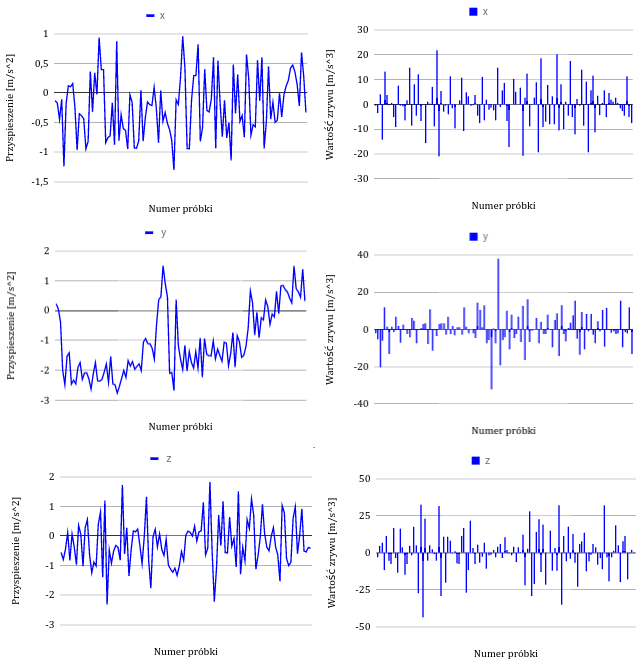
\includegraphics[width=16cm]{img/driving_analysis/12_5Hz_Przyspieszanie.png}
	\caption{Wykresy przyspieszenia i zrywu w trakcie przyspieszania przy częstotliwości próbkowania 12.5 Hz.
	\\Źródło: Twórczość własna}
	\label{fig:image_driving_analysis_test_12Hz}
\end{figure}

Jak widać, dane wydają się niekompletne, "poszatkowane", zwłaszcza te dotyczące zrywu. Po pierwszych testach postanowiono zrezygnować z brania pod uwagę przyspieszeń w osi Z ze względu na ich znikomy wkład w opis stylu jazdy kierowcy.

Następnym krokiem badań było sprawdzenie wpływu zwiększenia częstotliwości próbkowania o jeden krok - do 26 Hz. W przypadku tego testu skorygowano pomyłkę orientacji urządzenia tak, aby zwrot osi Y pokrywał się z kierunkiem jazdy na wprost. Pozostałe warunki orientacji pozostały bez zmian. Wyniki badań przedstawiono na rysunkach \ref{fig:image_driving_analysis_test_26Hz} i \ref{fig:image_driving_analysis_test_acc_26Hz}.

\begin{figure}[H]
	\centering
	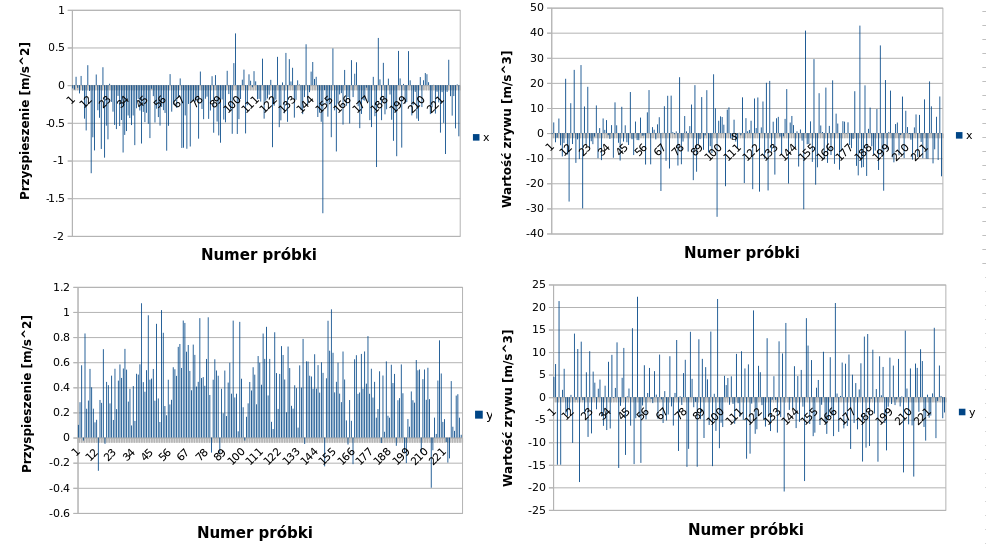
\includegraphics[width=18cm]{img/driving_analysis/stabilna_26.png}
	\caption{Wykresy przyspieszenia i zrywu w trakcie stabilnej jazdy przy częstotliwości próbkowania 26 Hz.
	\\Źródło: Twórczość własna}
	\label{fig:image_driving_analysis_test_26Hz}
\end{figure}

\begin{figure}[H]
	\centering
	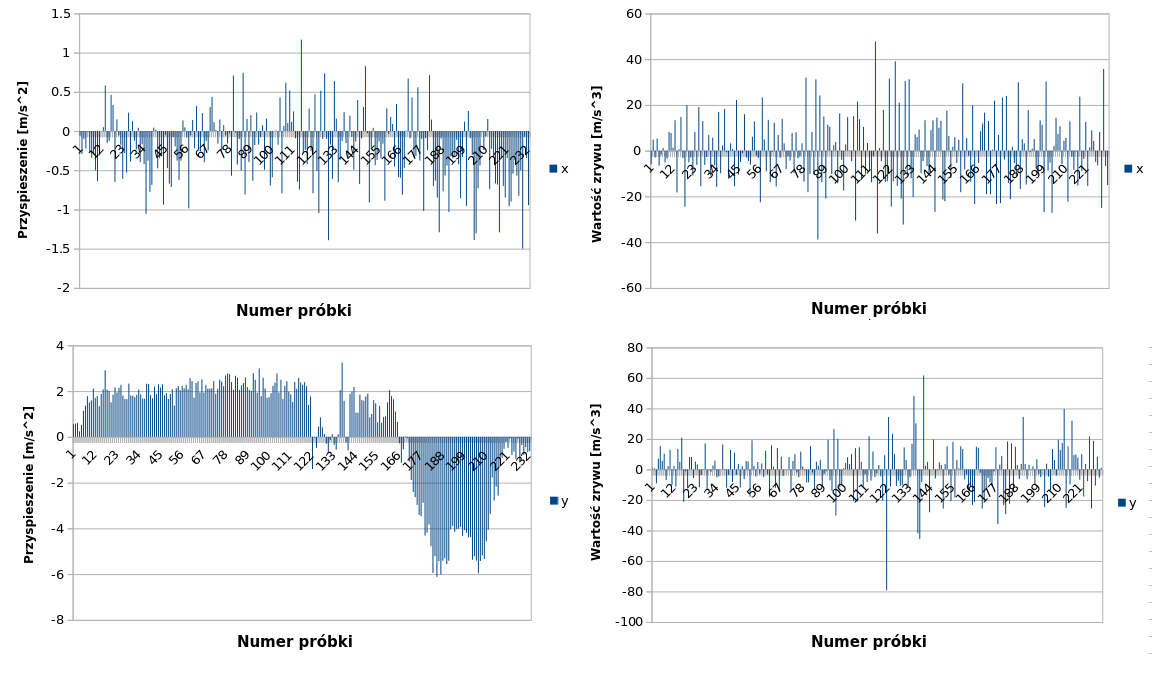
\includegraphics[width=18cm]{img/driving_analysis/Ostre_przyspieszenie_26Hz.png}
	\caption{Wykresy przyspieszenia i zrywu w trakcie agresywnego przyspieszania i hamowania przy częstotliwości próbkowania 26 Hz.
	\\Źródło: Twórczość własna}
	\label{fig:image_driving_analysis_test_acc_26Hz}
\end{figure}

\clearpage
Jak widać na przedstawionych powyżej rysunkach, wzrost częstotliwości bardzo pozytywnie wpłynął na zebrane dane w przypadku przyspieszenia, lecz wartość zrywu wciąż wydaje się niekompletna. Kolejnym wnioskiem jest fakt, iż zakresy dla agresywnego przyspieszania i hamowania są różne. Jest to oczekiwany wynik, gdyż zazwyczaj hamulce pojazdów są znacznie skuteczniejsze niż ich zdolność do przyspieszania. 

Po zebraniu kilku innych zestawów próbek, postanowiono dokonać dalszego zwiększenia częstotliwości próbkowania o kolejny krok do 52 Hz. Wyniki dla jazdy na wprost ze stałą prędkością przedstawiono na rysunku \ref{fig:image_driving_analysis_test_52Hz}.

\begin{figure}[H]
	\centering
	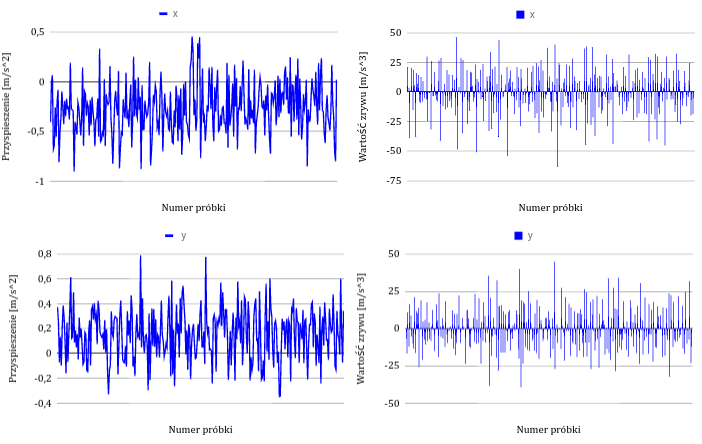
\includegraphics[width=15cm]{img/driving_analysis/stabilna_52.png}
	\caption{Wykresy przyspieszenia i zrywu w trakcie stabilnej jazdy przy częstotliwości próbkowania 52 Hz.
	\\Źródło: Twórczość własna}
	\label{fig:image_driving_analysis_test_52Hz}
\end{figure}

Na powyższym obrazku widać, że dane są już kompletne. Z tego powodu zdecydowano się na zastosowanie częstotliwości próbkowania wynoszącej 52 Hz. Dodatkowo jest to optymalny kompromis pomiędzy dokładnością danych, a czasem ich przetwarzania i niezbędną ilością pamięci w mikrokontrolerze do ich zgromadzenia. Pozostałe przypadki rozpatrywanych zachowań na drodze przedstawiono na rysunkach: \ref{fig:image_driving_analysis_test_acc_light_aggressive_52Hz} i \ref{fig:image_driving_analysis_test_acc_light_hard_lane_52Hz}.

\begin{figure}[H]
	\centering
	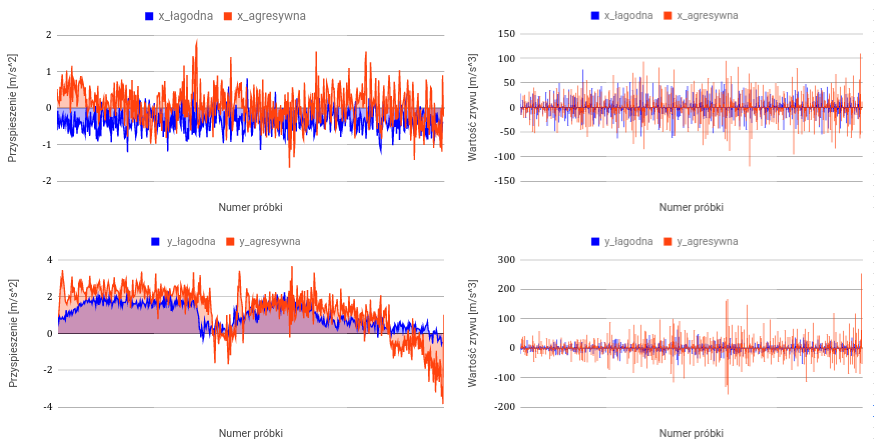
\includegraphics[width=16cm]{img/driving_analysis/zestawienie_lagodna_ostra-ruszanie.png}
	\caption{Zestawienie wykresów przyspieszenia i zrywu w trakcie łagodnego i agresywnego przyspieszania przy częstotliwości próbkowania 52 Hz.
	\\Źródło: Twórczość własna}
	\label{fig:image_driving_analysis_test_acc_light_aggressive_52Hz}
\end{figure}

\begin{figure}[H]
	\centering
	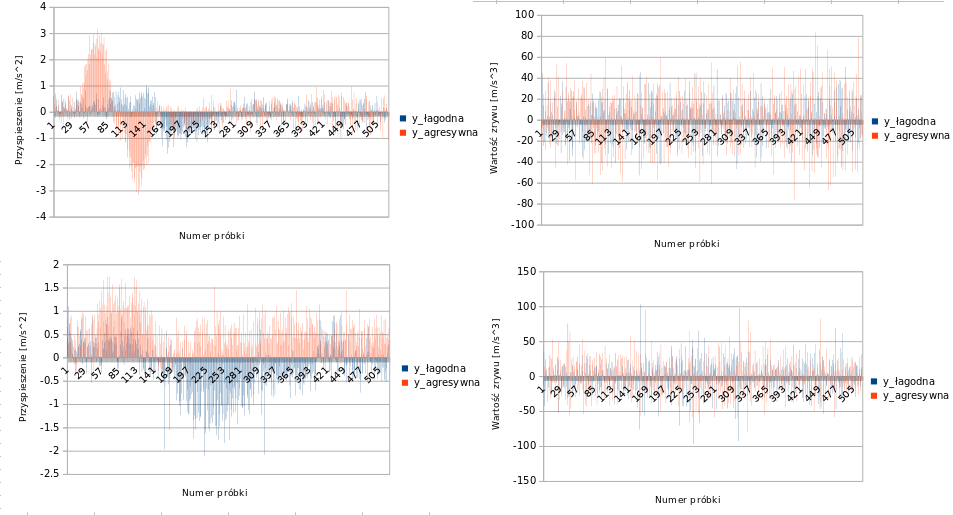
\includegraphics[width=16cm]{img/driving_analysis/zestawienie_ostra_lagodna.png}
	\caption{Zestawienie wykresów przyspieszenia i zrywu w trakcie łągodnej i agresywnej zmiany pasa przy częstotliwości próbkowania 52 Hz.
	\\Źródło: Twórczość własna}
	\label{fig:image_driving_analysis_test_acc_light_hard_lane_52Hz}
\end{figure}


\clearpage
Na podstawie danych przedstawionych na powyższych rysunkach otrzymano następujące wnioski:

\begin{itemize}
\item Dane nie posiadają znaczącego czynnika losowego w postaci szumu, zatem nie jest konieczne ich dodatkowe filtrowanie
\item Wartość i rozkład przyspieszenia w obrębie okna czasowego zbierania próbek bardzo wyraźnie informuje o rodzaju wykonywanego manewru.
\item Wartość zrywu jest w przybliżeniu symetryczna względem wartości zero. Oznacza to, że jego średnia wartość w całym zakresie próbek jest bliska zeru.
\item Wraz ze wzrostem poziomu agresji w stylu jazdy, wartość wariancji zrywu oraz moduł przyspieszenia średniego rośnie. 
\end{itemize}

Ostatni wniosek jest szczególnie istotny dla zaproponowanego w niniejszej pracy algorytmu oceny stylu jazdy kierowcy. 

\section{Metoda zastosowana w pracy}

Metoda powstała na podstawie analizy wniosków z podrozdziału \ref{experiments}. W swych podstawach wykorzystuje ona przyspieszenie oraz wariancję zrywu. Jedynym  jej założeniem jest konieczność odpowiedniej orientacji urządzenia względem kierunku jazdy. Mianowicie, jak już zostało wcześniej wspomniane, oś Y akcelerometru musi pokrywać się z kierunkiem jazdy na wprost, a oś Z powinna być skierowana prostopadle do podłoża. Algorytm jest następujący:

\begin{enumerate}
\item Pobierz wartości przyspieszeń zakolejkowane w akcelerometrze z okresu pomiędzy próbkami lokalizacji (domyślnie 10 sekund).
\item Dla otrzymanego zbioru danych wylicz wartości zrywu dla osi X i Y.
\item Podziel zbiór próbek na okna czasowe o szerokości 0.5 sekundy. Zastosowanie tego kroku pozwala na kwantyzację czasową w celu uśrednienia danych. Szerokość okna została dobrana na podstawie wyników badań z podrozdziału \ref{experiments}, w celu zachowania jak największej ilości szczegołów w oknie uśredniającym.
\item Dla każdego okna wylicz przyspieszenia średnie w osiach X i Y, a także wariancję zrywów w tych osiach.
\item Normalizuj każdy z powyższych parametrów, dzieląc go przez pewien dobrany eksperymentalnie próg, wyróżniając przy tym przyspieszanie od hamowania w kierunku jazdy na wprost, ze względu na konieczność zastosowania odrębnych progów normalizujących.
\item Od każdego ze znormalizowanych parametrów odejmij wartość stałą stanowiącą jego odpowiednik dla jazdy ze stałą prędkością. Krok ten jest efektem rozumowania, iż agresywny styl jazdy jest niejako stylem łagodnym, z nałożonym na niego pewnym wzorcem ostrej jazdy. Dzięki niemu, oceniany jest jedynie zmienny wpływ czynnika "agresywności", bez uwzględniania wpływu od jazdy ze stałą prędkością.
\item Oblicz ocenę złożoną dla każdej z osi X i Y. Ocena ta stanowi średnią ważoną składowych średniego przyspieszenia znormalizowanego i znormalizowanej wariancji zrywu z wagami wynoszącymi odpowiednio 1 i 2. Wynika to z faktu, iż na podstawie obserwacji danych przedstawionych w podrozdziale \ref{experiments}, wariancja zrywu wykazuje lepszą zdolność do klasyfikacji konkretnych manewrów drogowych.
\item Wyznaczenie oceny dla próbki jako średniej arytmetycznej ocen z osi X i Y.
\item Wyznaczenie oceny całej trasy jako średniej ważonej ocen każdej próbki należącej do tej trasy.
\end{enumerate}

Algorytm ten przedstawiono na rysunku \ref{fig:image_driving_analysis_alghoritm}.

\begin{figure}[H]
	\centering
	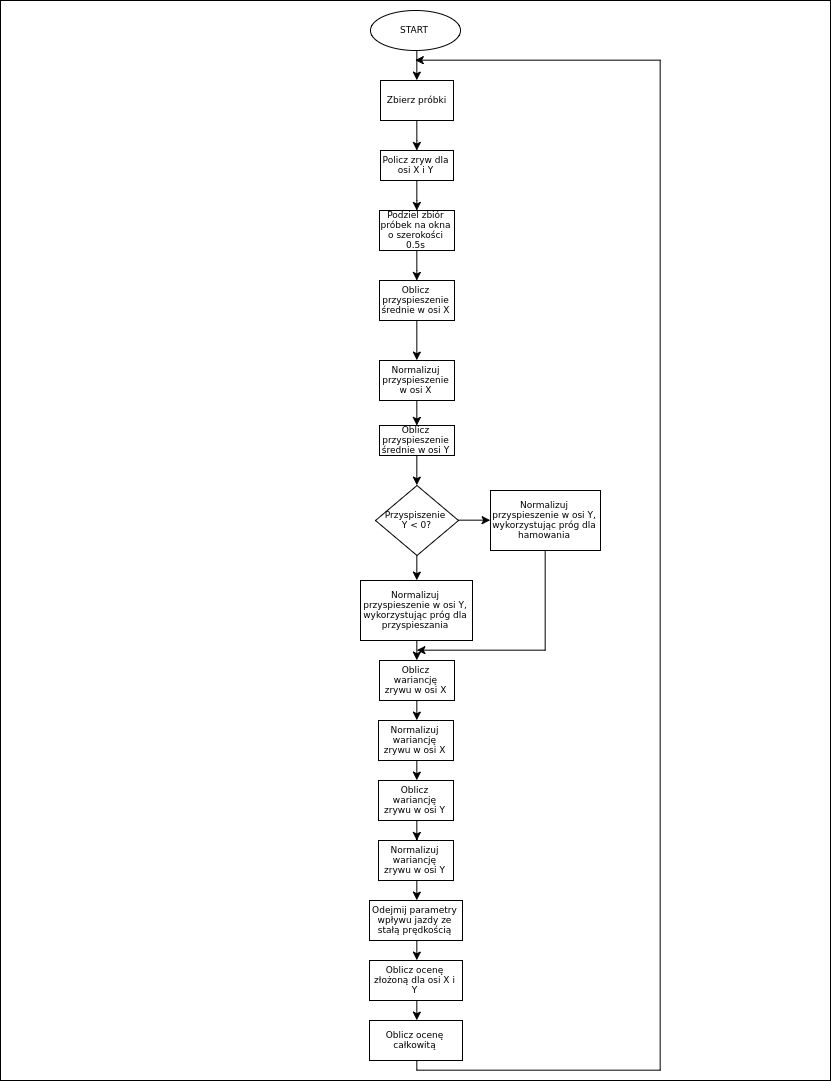
\includegraphics[width=15cm]{img/driving_analysis/driving_analysis.png}
	\caption{Algorytm oceny stylu jazdy. Źródło: Twórczość własna}
	\label{fig:image_driving_analysis_alghoritm}
\end{figure}

Wyliczona ocena zawiera się w przedziale $[0.00; 1,00]$, gdzie wynik 0.00 oznacza jazdę łagodną, a 1.00 - bardzo agresywną. Na stronie internetowej są one interpretowane w skali procentowej, gdzie 0\% oznacza bardzo agresywną jazdę, a 100\% bardzo spokojną. Ponadto, dodatkowo są one wizualizowane na kolorowym pasku, którego barwa płynnie określa ocenę stylu jazdy.


\section{Rezultaty}

W ramach dokonywania testów skuteczności algorytmu, wykonano kilka przejazdów samochodem po różnych trasach. Jedną z wielu tras przedstawiono na rysunku \ref{fig:image_driving_analysis_alghoritm_track_1}.

\begin{figure}[H]
	\centering
	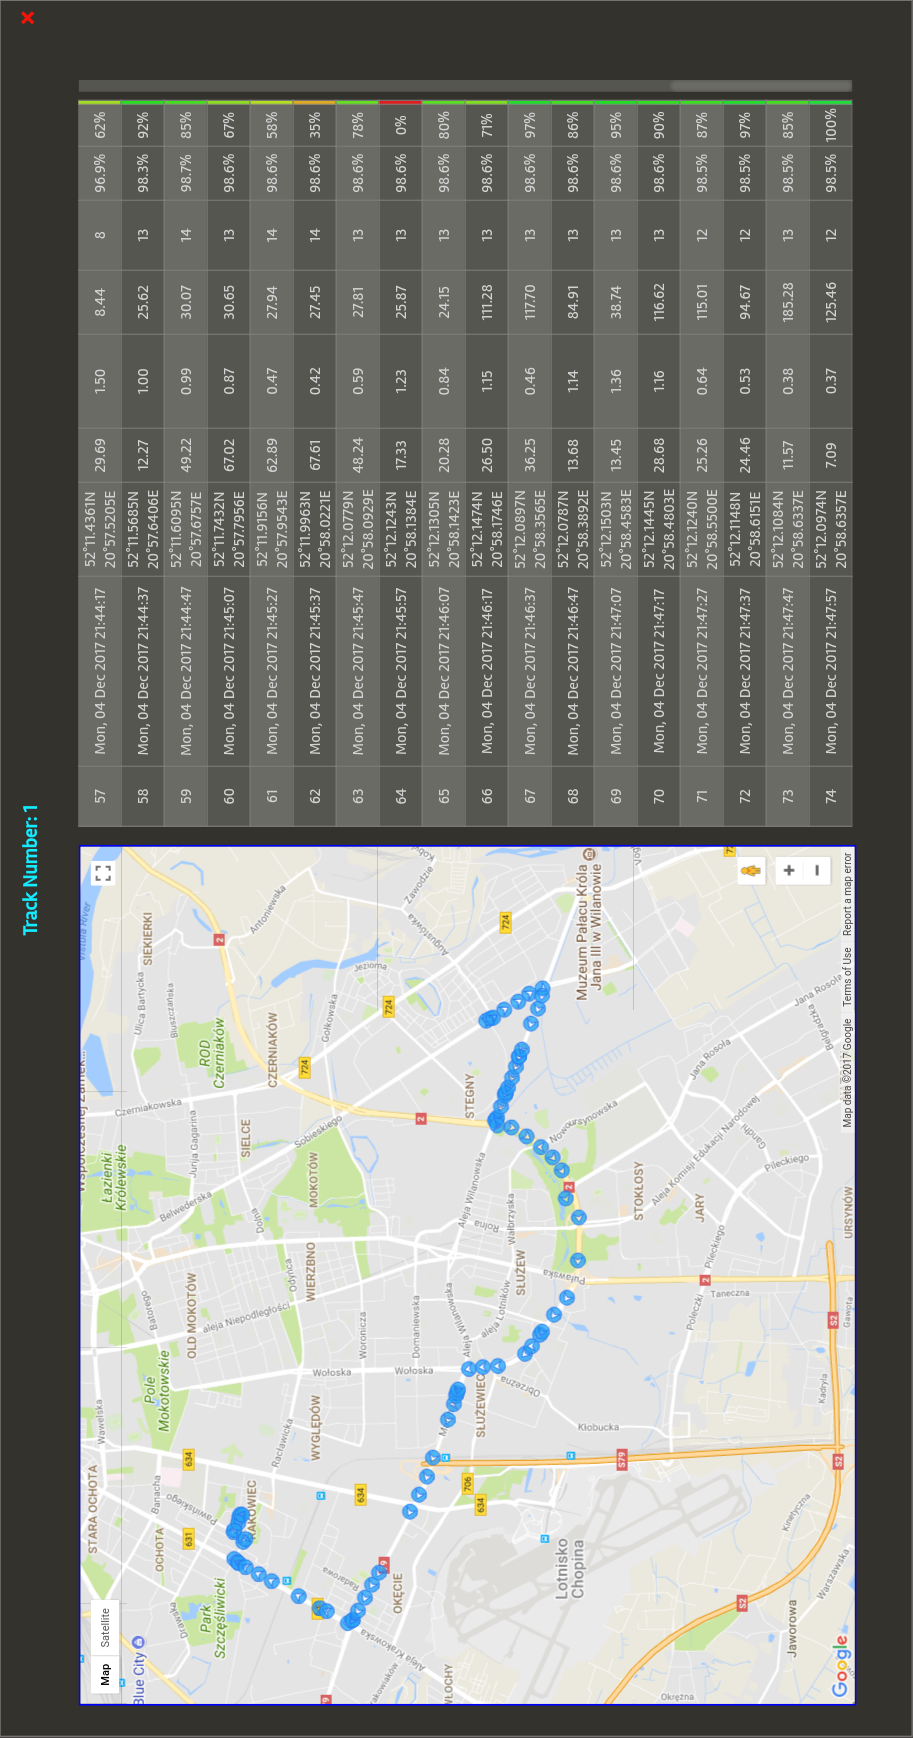
\includegraphics[height=19cm, width=13cm]{img/driving_analysis/test_track_1.png}
	\caption{Trasa próbna nr 1. Źródło: Twórczość własna}
	\label{fig:image_driving_analysis_alghoritm_track_1}
\end{figure}


Poniższa trasa została pokonana w Warszawie. Start nastąpił o godzinie 21:41:57 z ulicy Egejskiej. Poruszano się ulicą Sobieskiego w kierunku Wilanowa, następnie dokonano skrętu w ul. Wilanowską w kierunku zachodnim aż do skrzyżowania z Doliną Służewiecką. Przejazd do tego momentu był łagodny, bez ostrych zmian pasów czy przyspieszeń. Wyniki przedstawiono na rysunku \ref{fig:image_driving_analysis_alghoritm_track_1_part_1}.

\begin{figure}[H]
	\centering
	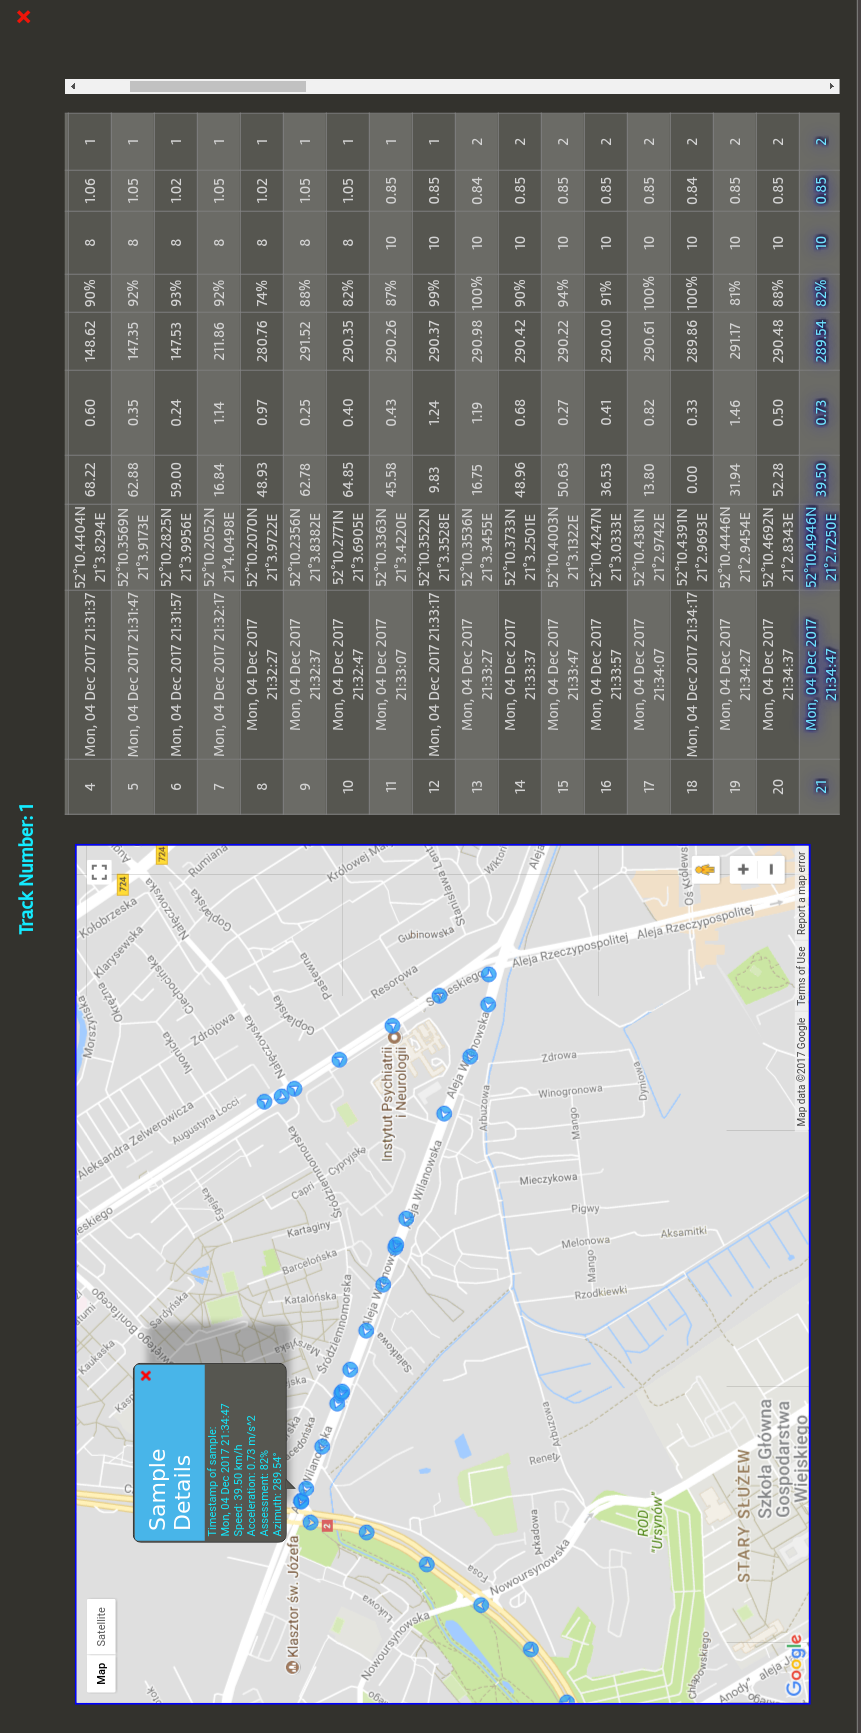
\includegraphics[height=19cm, width=13cm]{img/driving_analysis/test_track_1_lagodna.png}
	\caption{Trasa próbna nr 1 - pierwsza częśś trasy. Źródło: Twórczość własna}
	\label{fig:image_driving_analysis_alghoritm_track_1_part_1}
\end{figure}

Następnie skręcono w Dolinę Slużewiecką, która przeszła w ulicę Rzymowskiego aż do skrzyżowania z ulicą Marynarską. Niewiele po rozpoczęciu poruszania się Doliną Służewiecką, dokonano zwiększenia nieco dynamiki jazdy. Polegała ona na zwiększeniu przyspieszania oraz kilkukrotnym zmianom pasów, jednak nie w stopniu który można by określić agresywnym, bądź niebezpiecznym. Przedstawiono to na rysunku \ref{fig:image_driving_analysis_alghoritm_track_1_part_2}.

\begin{figure}[H]
	\centering
	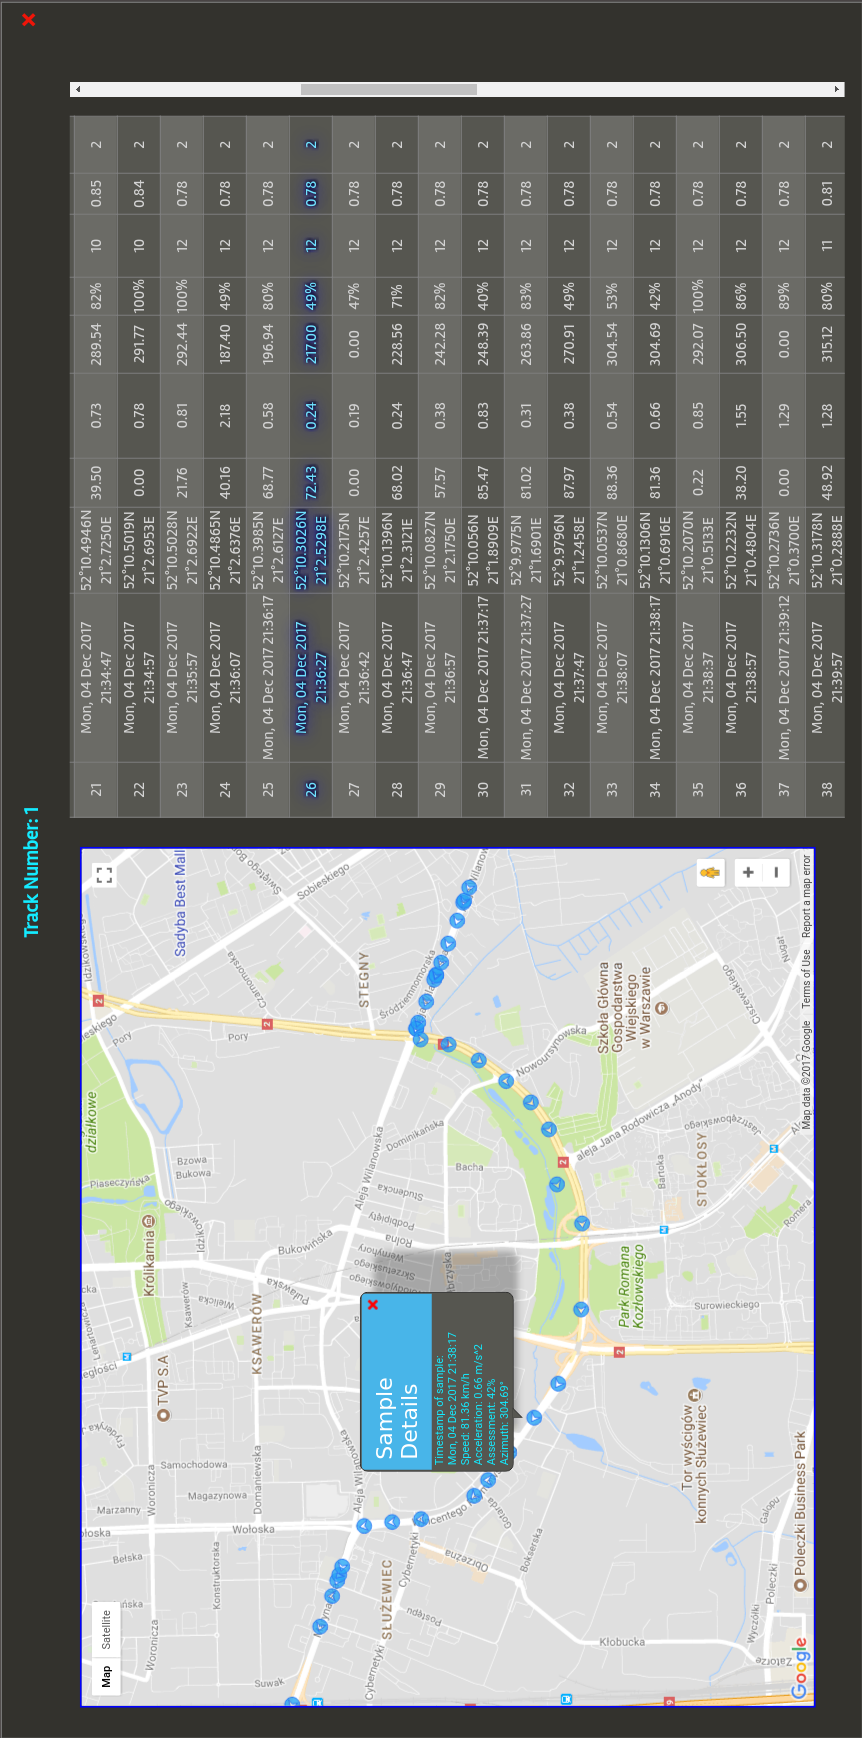
\includegraphics[height=19cm, width=13cm]{img/driving_analysis/test_track_part_2.png}
	\caption{Trasa próbna nr 1 - druga część trasy. Źródło: Twórczość własna}
	\label{fig:image_driving_analysis_alghoritm_track_1_part_2}
\end{figure}

Kolejnym etapem był zjazd w ulicę Marynarską i jazda nią aż do Alei Krakowskiej. Od pewnego momentu pierwszej z nich, mniej więcej na wysokości trasy S79 występuje podwyższenie dopuszczalnej prędkości do 80 km/h. Tam dokonano testów agresywnej jazdy. Polegały one na cyklicznym, chwilowym, lecz częstym, mocnym przyspieszaniu oraz gdy warunki na to pozwalały - hamowaniu. Ostre hamowanie nastąpiło tuż przed zjazdem w ulicę Aleja Krakowska. Wyniki testów przedstawiono na rysunku \ref{fig:image_driving_analysis_alghoritm_track_1_part_3}.

\begin{figure}[H]
	\centering
	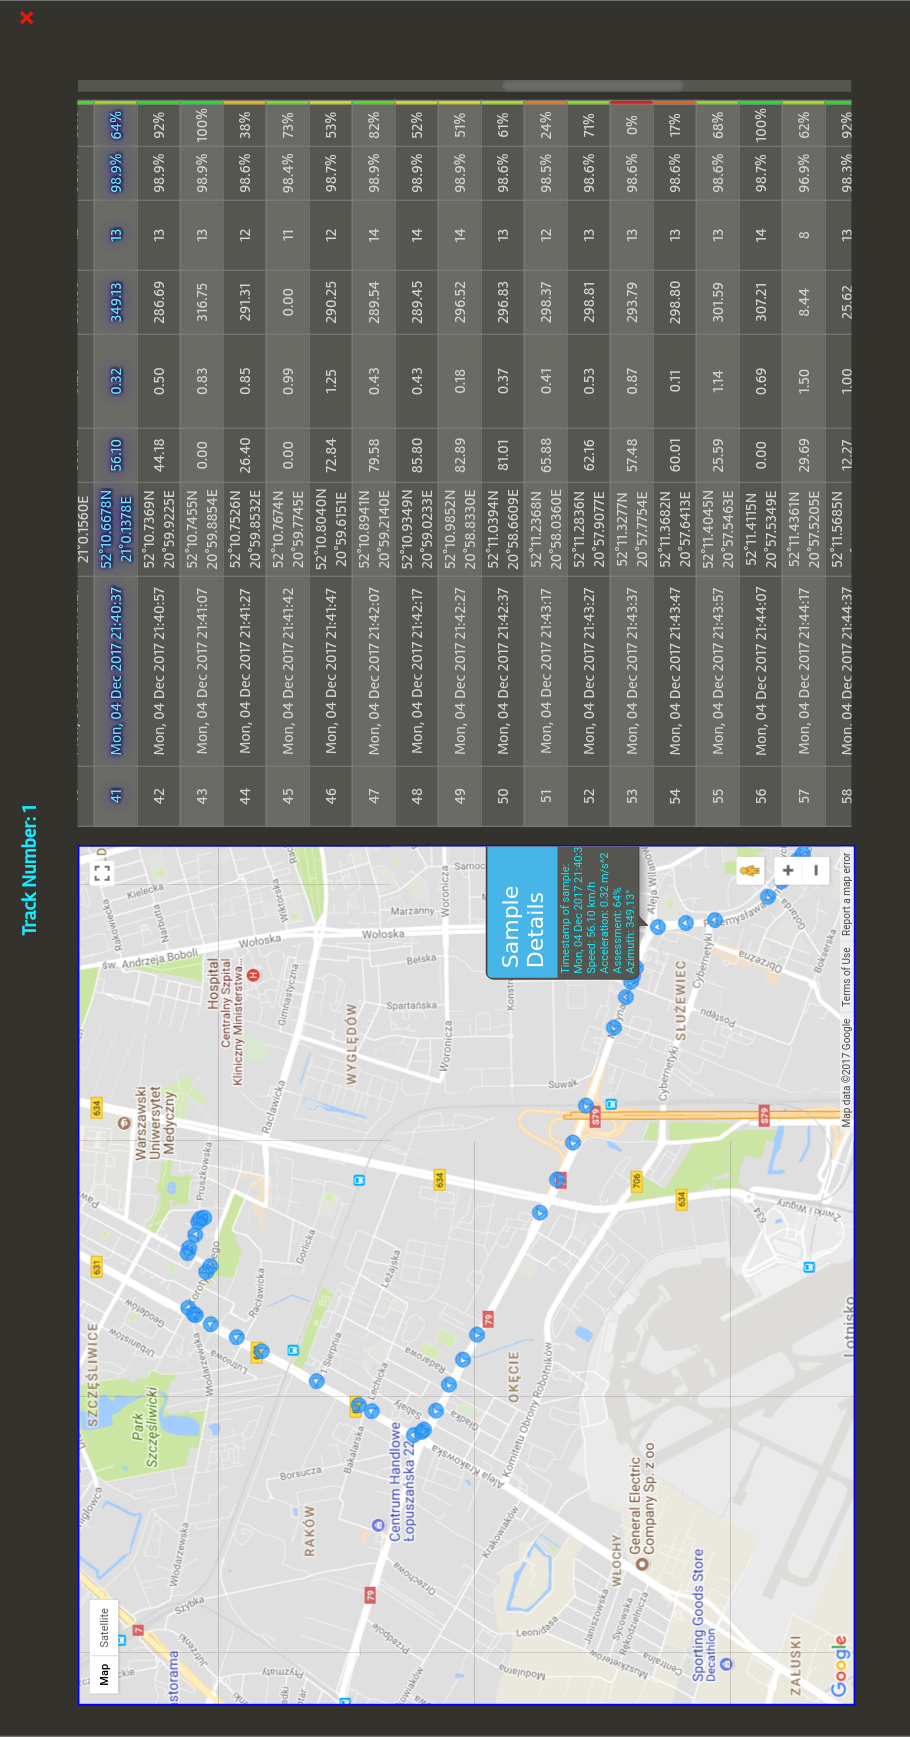
\includegraphics[height=19cm, width=13cm]{img/driving_analysis/test_track_part_3.png}
	\caption{Trasa próbna nr 1 - trzecia część trasy. Źródło: Twórczość własna}
	\label{fig:image_driving_analysis_alghoritm_track_1_part_3}
\end{figure}

Ostatnia część trasy - przejazd ulicami: Aleja Krakowska, Korotyńskiego i Pruszkowska przebiegł już łagodnie, co przedstawiono na rysunku \ref{fig:image_driving_analysis_alghoritm_track_1_part_4}.

\begin{figure}[H]
	\centering
	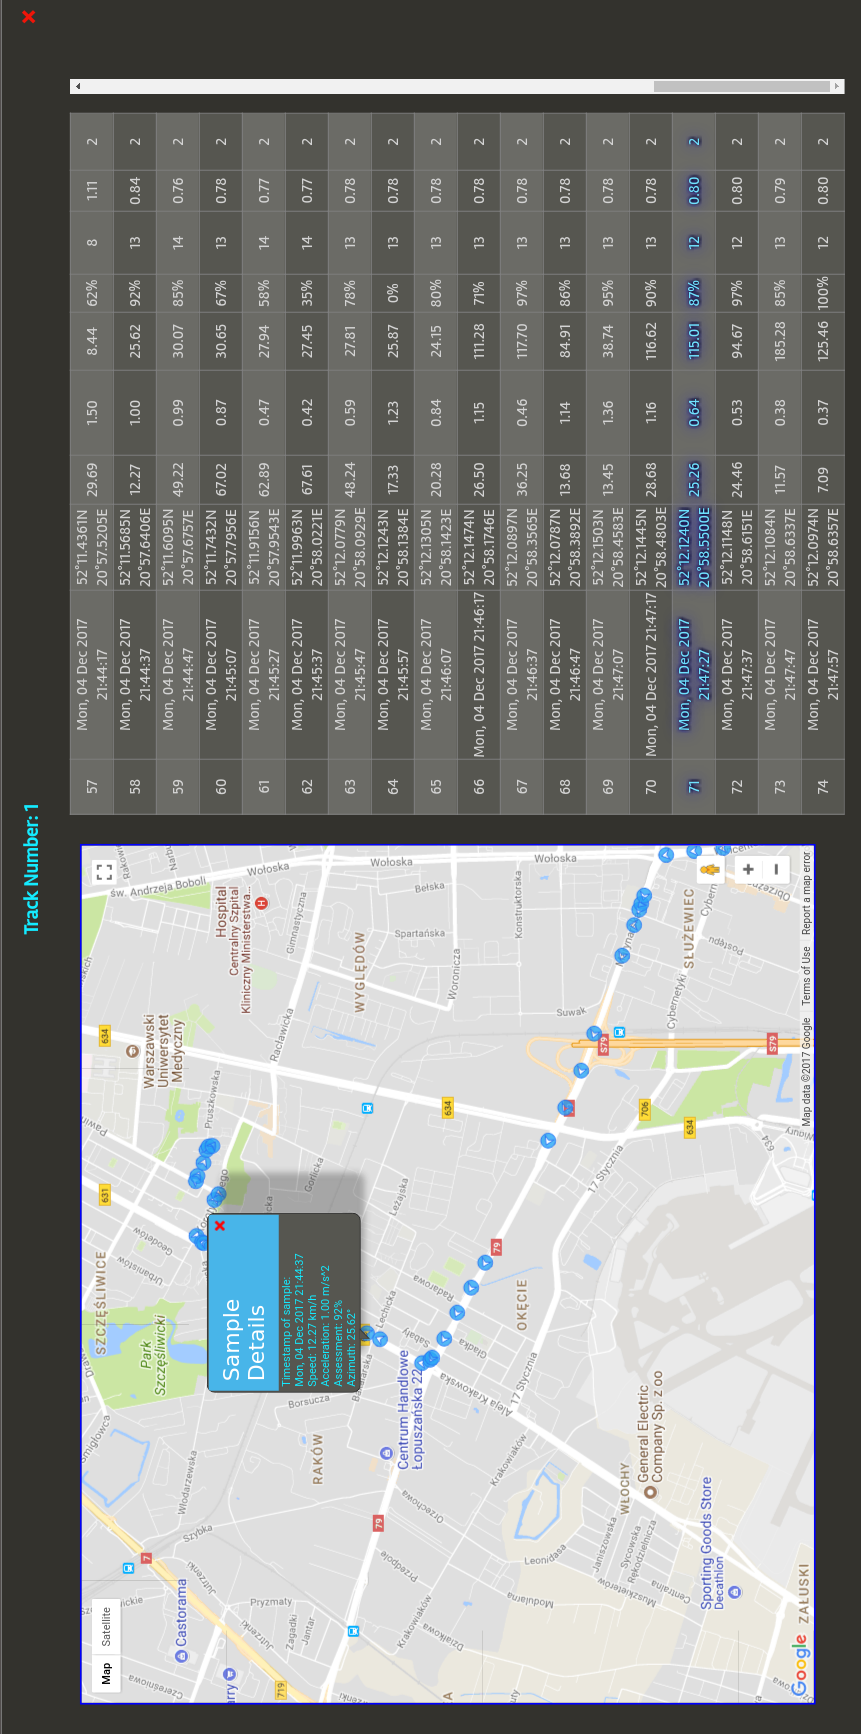
\includegraphics[height=19cm, width=13cm]{img/driving_analysis/test_track_part_4.png}
	\caption{Trasa próbna nr 1 - czwarta część trasy. Źródło: Twórczość własna}
	\label{fig:image_driving_analysis_alghoritm_track_1_part_4}
\end{figure}

Jak widać, dane zgromadzone w bazie danych, przypisane do tej trasy odzwierciedlają sposób jazdy, co dowodzi skuteczności algorytmu.
